% ****** Start of file apssamp.tex ******
%
%   This file is part of the APS files in the REVTeX 4.2 distribution.
%   Version 4.2a of REVTeX, December 2014
%
%   Copyright (c) 2014 The American Physical Society.
%
%   See the REVTeX 4 README file for restrictions and more information.
%
% TeX'ing this file requires that you have AMS-LaTeX 2.0 installed
% as well as the rest of the prerequisites for REVTeX 4.2
%
% See the REVTeX 4 README file
% It also requires running BibTeX. The commands are as follows:
%
%  1)  latex apssamp.tex
%  2)  bibtex apssamp
%  3)  latex apssamp.tex
%  4)  latex apssamp.tex
%
\documentclass[%
 reprint,
%superscriptaddress,
%groupedaddress,
%unsortedaddress,
%runinaddress,
%frontmatterverbose, 
%preprint,
%preprintnumbers,
nofootinbib,
%nobibnotes,
%bibnotes,
 amsmath,amssymb,
 aps,
%pra,
%prb,
%rmp,
%prstab,
%prstper,
%floatfix,
]{revtex4-2}
\usepackage{lipsum}
\usepackage{caption}
\usepackage{subcaption}
\usepackage{siunitx}
\usepackage{gensymb}
\usepackage{booktabs}
\usepackage{multirow}
\sisetup{separate-uncertainty=true}
\usepackage{graphicx}% Include figure files
\usepackage{dcolumn}% Align table columns on decimal point
\usepackage{bm}% bold math
\usepackage{hyperref}% add hypertext capabilities
\usepackage{xcolor}
\hypersetup{
	colorlinks,
	linkcolor={blue},
	citecolor={red},
	urlcolor={purple}
}
%\usepackage[mathlines]{lineno}% Enable numbering of text and display math
%\linenumbers\relax % Commence numbering lines

%\usepackage[showframe,%Uncomment any one of the following lines to test 
%%scale=0.7, marginratio={1:1, 2:3}, ignoreall,% default settings
%%text={7in,10in},centering,
%%margin=1.5in,
%%total={6.5in,8.75in}, top=1.2in, left=0.9in, includefoot,
%%height=10in,a5paper,hmargin={3cm,0.8in},
%]{geometry}

\begin{document}

\preprint{APS/123-QED}

\title{Experiments in Fiber Optics}% Force line breaks with \\
%\thanks{A footnote to the article title}%

\author{Maitrey Sharma}
\email{maitrey.sharma@niser.ac.in}
\thanks{\\Roll No.: 1911093}
% \altaffiliation[Also at ]{Physics Department, XYZ University.}%Lines break automatically or can be forced with \\
%\author{Second Author}%
% \email{Second.Author@institution.edu}
\affiliation{%
 School of Physical Sciences, National Institute of Science Education and Research, HBNI, Jatni-752050, India.\\
 %This line break forced with \textbackslash\textbackslash
}%
%\collaboration{MUSO Collaboration}%\noaffiliation

%\author{Charlie Author}
% \homepage{http://www.Second.institution.edu/~Charlie.Author}
%\affiliation{
% Second institution and/or address\\
% This line break forced% with \\
%}%
%\affiliation{
% Third institution, the second for Charlie Author
%}%
%\author{Delta Author}
%\affiliation{%
% Authors' institution and/or address\\
% This line break forced with \textbackslash\textbackslash
%}%

%\collaboration{CLEO Collaboration}%\noaffiliation

\date{\today}% It is always \today, today,
             %  but any date may be explicitly specified

\begin{abstract}
In this experiment, we have undertake various experiments concerning optical fibers, the backbone of modern communications systems. We begin by understanding  the handling of the fibers using tools and how to prepare them for experiments. We classify between different kinds of optical fibers (single-mode and multi-mode) and carefully explore how they are affected differently in various experiments. We calculate numerical apertures, mode-field diameters, and micro- and macro-bending losses in the fibers to build a greater understanding of their working.
%\item[Usage]
%econdary publications and information retrieval purposes.
%\item[Structure]
%You may use the \texttt{description} environment to structure your abstract;
%use the optional argument of the \verb+\item+ command to give the category of each item. 
%\end{description}
\end{abstract}

%\keywords{Suggested keywords}%Use showkeys class option if keyword
                              %display desired
\maketitle

%\tableofcontents

\section{Introduction}


In the early 1840s Paris, Daniel Colladon and Jacques Babinet first demonstrated the guiding of light by refraction and by the 19th century, a team of doctors from Vienna were able to guide light through bent glass rods to illuminate body cavities. Over the next century practical applications followed and in 1953, Dutch scientist Bram van Heel first demonstrated image transmission through bundles of optical fibers with a transparent cladding. 


\begin{figure}
	\centering
	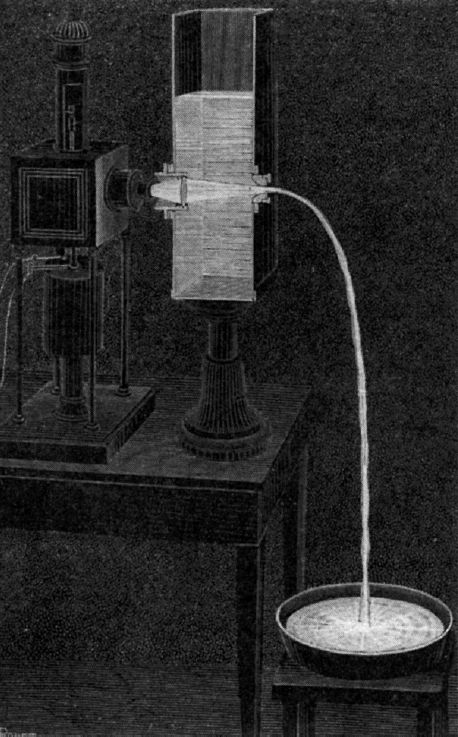
\includegraphics[scale = 0.65]{colladon}
	\caption{An illustration of Colladon's \textit{light fountain} from one of his publications.}
\end{figure}

Today, optical fibers form the backbone of our communications systems, permitting transmission of data over longer distances and at higher bandwidths (data transfer rates) than electrical cables. They suffer less loss and suffer less electromagnetic interference than their metal counterparts. Their usage extends beyond data transmission to various specialized instrumentations like sensors and lasers.

Optical fibers typically include a core surrounded by a transparent cladding material with a lower index of refraction. Light is kept in the core by the phenomenon of total internal reflection which causes the fiber to act as a waveguide. Fibers that support many propagation paths or transverse modes are called \textit{multi-mode fibers}, while those that support a single mode are called \textit{single-mode fibers}.



\section{Objectives}
There are several major objectives that will be achieved as part of this experiment. They are:
\begin{enumerate}
	\item The preparation of an optical fiber for experiments will be understood.
	\item We will calculate numerical aperture of both single-mode and multi-mode fibers.
	\item We will calculate the mode field diameter of a single-mode fiber.
	\item We will be studying the effects of microbending loss and will explore its applications in sensing for multi-mode fibers.
	\item Finally, we will also be studying the mechanics of bend-induced in a single-mode fiber.
\end{enumerate}

\section{Experimental setup}

The setup uses an optical breadboard to mount all the necessary equipment, which includes a helium-neon laser source, aligners for the source (see Figure \ref{fig:hene}), a microscopic objective (40X), microscopic objective holder, transnational stages with chucks (fiber positioners) mounted on them, a photo-detector connected to a multimeter, a photo-detector holder, and posts and holders as needed. In addition to this, along the single-mode and multi-mode fibers, we used a fiber stripper to remove the cladding of the fibers, a fiber cutter and an index matching liquid to clean the fiber ends before coupling them with the laser. 
\begin{figure}
	\centering
	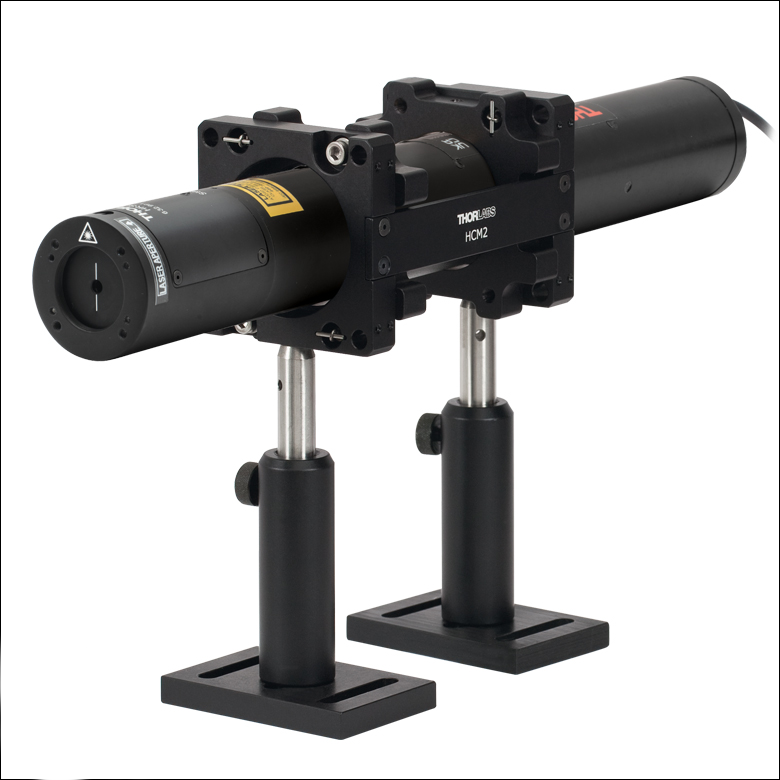
\includegraphics[scale = 0.3, trim=4 4 4 4,clip]{mountedLaser}
	\caption{He-Ne laser with aligners in place}
	\label{fig:hene}
\end{figure}


\begin{figure}
	\centering
	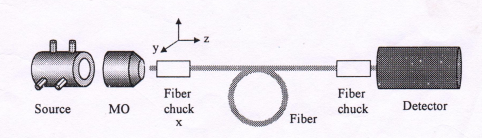
\includegraphics[scale=0.65]{setup}
	\caption{Experimental setup for launching light from a laser diode into an optical fiber using an MO.}
	\label{fig:setup}
\end{figure}


The final setup, in its idealized state, looks like as shown in Figure \ref{fig:setup}.


Our initial setup was not optimal. The mounts were wobbly and it was difficult to stabilize them and maneuvering them precise alignment which is needed for coupling the fiber with the laser. In the setup that we inherited from the previous group who worked there was only one holder (or aligner) to adjust the laser source, but we discovered that it was not stable enough. To solve this, we fitted one more aligner but that made the whole source to rigid, leaving us out of any way to align it. 

\subsection*{Our Innovation to improve the setup}
The process of alignment consists of four components that need to be aligned with each other: the source itself, the microscopic objective (MO), the fiber, and then the detector. Here, the alignment of source with the MO and that of fiber with the detector is trivial. However, aligning the MO with the fiber requires precision. To reacquire fine control to align the our setup, we mounted two mirrors in the Z-fold configuration (see Figure \ref{fig:zfold}). Now we could use the kinetic mounts of the mirrors we used (see Figure \ref{fig:kinetic}) for precise alignment. We also used apertures (irises) to align the laser further down the optical breadboard. Through this z-fold configuration we created a very robust setup which was then easily aligned.

There were some more problems with the setup, such as faulty translation stages, due to which we had to skip few experiments, whereas nonavailability of a different type of laser source meant we could not do some specific experiments (more in Section \ref{sec:Disc}).

\begin{figure}
	\centering
	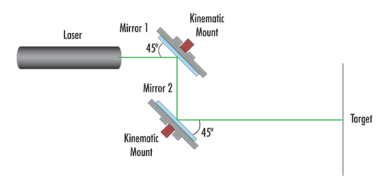
\includegraphics{zfold}
	\caption{The Z-fold configuration in laser alignment techniques}
	\label{fig:zfold}
\end{figure}

\begin{figure}
	\centering
	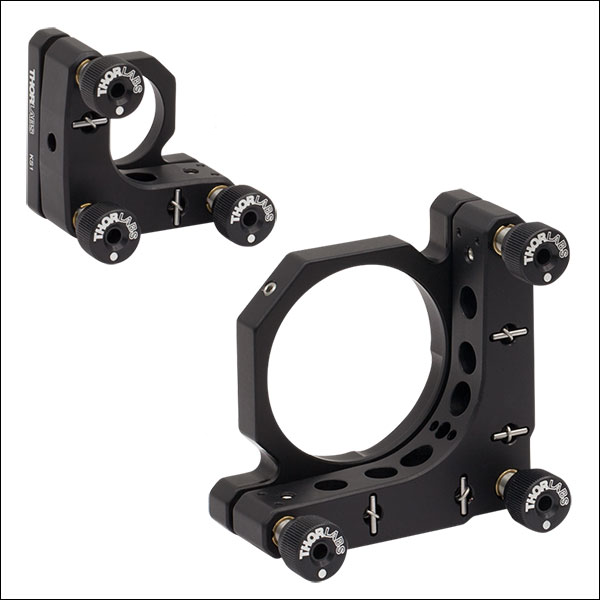
\includegraphics[scale=0.3, trim=4 4 4 4,clip]{kineticMirror}
	\caption{Mirrors used in the z-fold configuration with kinetic mounts}
	\label{fig:kinetic}
\end{figure}

\section{The Experiments}
\subsection{Fiber-end preparation and coupling}
Before taking any measurements, we need to ensure that
the end-faces of the fibre are perpendicular to the axis of
the fibre. We strip the cladding on both the fibre ends, over a
very short distance. Then we clean it with isopropyl alcohol.
Then for end preparation a high precision cleaver was used.
If required, a very small amount of oil (or any high refractive
index fluid) might be put on the ends to remove cladding
modes.


For coupling, we launch light from the laser diode onto the
microscope objective (MO). The MO acts a lens, wherein the
parallel rays of light from the laser are focused on a spot and
transmitted to the optical fibre. To couple light from the
source to the fibre, we need to ensure that the laser, MO and
the fibre lie at the same vertical level. For this we measure
the height of laser output using a scale at different distances
and ensure it is the same. We also measure the height of the
MO and fibre and keep it at the same level. We adjust the
fine knobs on the translational stage until we get the maxi-
mum output.

\begin{figure}
	\centering
	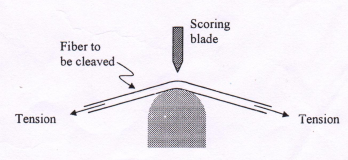
\includegraphics[scale=0.65]{cleave}
	\caption{Controlled-fracture of an optical fiber for its end-preparation through bend, score and
		break techniaue.}
	\label{fig:cleave}
\end{figure}

\begin{figure}
	\centering
	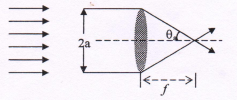
\includegraphics[scale = 0.65]{MO}
	\caption{lens representing a MO of focal length f and numerical aperture $ \sin \theta_a $}
	\label{fig:mo}
\end{figure}


\begin{figure}
	\centering
	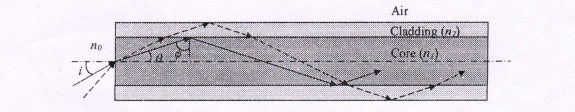
\includegraphics[scale=0.55]{coupling}
	\caption{Ray diagram illustrating the propagation of guided and cladding modes in an optical fiber}
	\label{fig:coupling}
\end{figure}

\subsection{Numerical Aperture measurements}
In simplest terms, numerical aperture is a measurement of the ability of an optical fiber to capture light. All fibers have acceptance angle (which forms the acceptance cone of the guided ray). The numerical aperture (NA) of a fiber is defined as the
sine of the largest angle an incident ray can have for total
internal reflectance in the core. Rays launched outside the
angle specified by a fiber’s NA will excite radiation modes of
the fiber.

Therefore, we can define numerical aperture quantitatively as
\begin{equation}\label{eq:NA}
	NA = \sin i_m = \sqrt{n_1^2 - n_2^2}
\end{equation}
where $ n_1 $ and $ n_2 $ are the refractive indices of the core and the cladding, respectively. Figure \ref{fig:na} shows the geometrcal ray path of a particular meridional ray in a step index multi-mode fiber.

The NA of the fiber is determined by measuring the angular dependance of the far field of the fiber. The far-field
of the fiber represents the field distribution at any distance
$ z \gg (2a)^2 / \lambda $ where $ a $ is the core radius of the fiber and $ \lambda $
is the operating wavelength. The semi-angle corresponding
to 5\% level of far field intensity maximum is the acceptance
angle. The acceptance angle is given by:
\begin{equation}\label{eq:sinNA}
	i_m = \dfrac{\theta_2 - \theta_1}{2}
\end{equation}
\begin{figure}
	\centering
	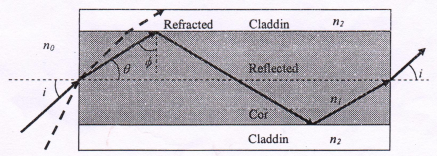
\includegraphics[scale=0.6]{na}
	\caption{A meridional ray entering a step index optical fiber at an angle $ i< i_m $ gets
		guided through the fiber, and comes out at the same angle $ i $ from the output end of the
		fiber. Rays incident at angles $ > i $, will get refracted into the cladding, eventually loosing
		all their energy in the cladding.}
	\label{fig:na}
\end{figure}

\begin{figure}
	\centering
	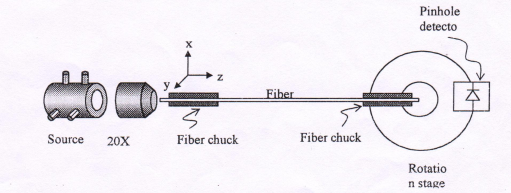
\includegraphics[scale = 0.5]{mm-NA}
	\caption{Experimental setup for scanning the far-field intensity distribution of a fiber using a rotational translation stage.}
	\label{fig:mm-na}
\end{figure}
\subsubsection*{\textbf{General Procedure}}
\begin{enumerate}
	\item The detector is mounted on a rotational stage.
	\item After end preparation and coupling, the maximum
	output is checked such that it lies at the $ 0 \degree $ of the rotational stage.
	\item The detector is rotated and the output is recorded.
	\item The angle $ i_m $ at which intensity drops to 5\% of the
	maximum value is measured and the acceptance angle is calculated.
\end{enumerate}

\subsubsection{Single-mode fiber}
For single-mode fiber, we find that the intensity variation with detector being rotated through an angle followed the Gaussian curve. We found the intersection points with the 5\% percent of the maximum intensity level at $ \theta_1 =  -0.17897$ and $ \theta_2 = 0.16694 $. Using equation \ref{eq:sinNA}, we got $ \sin i_m = 0.172 $ which is close to the actual value of $ 0.1 $ for the numerical aperture. This whole is plotted, fitted and labeled in Figure \ref{fig:smNA}.


\begin{figure}
	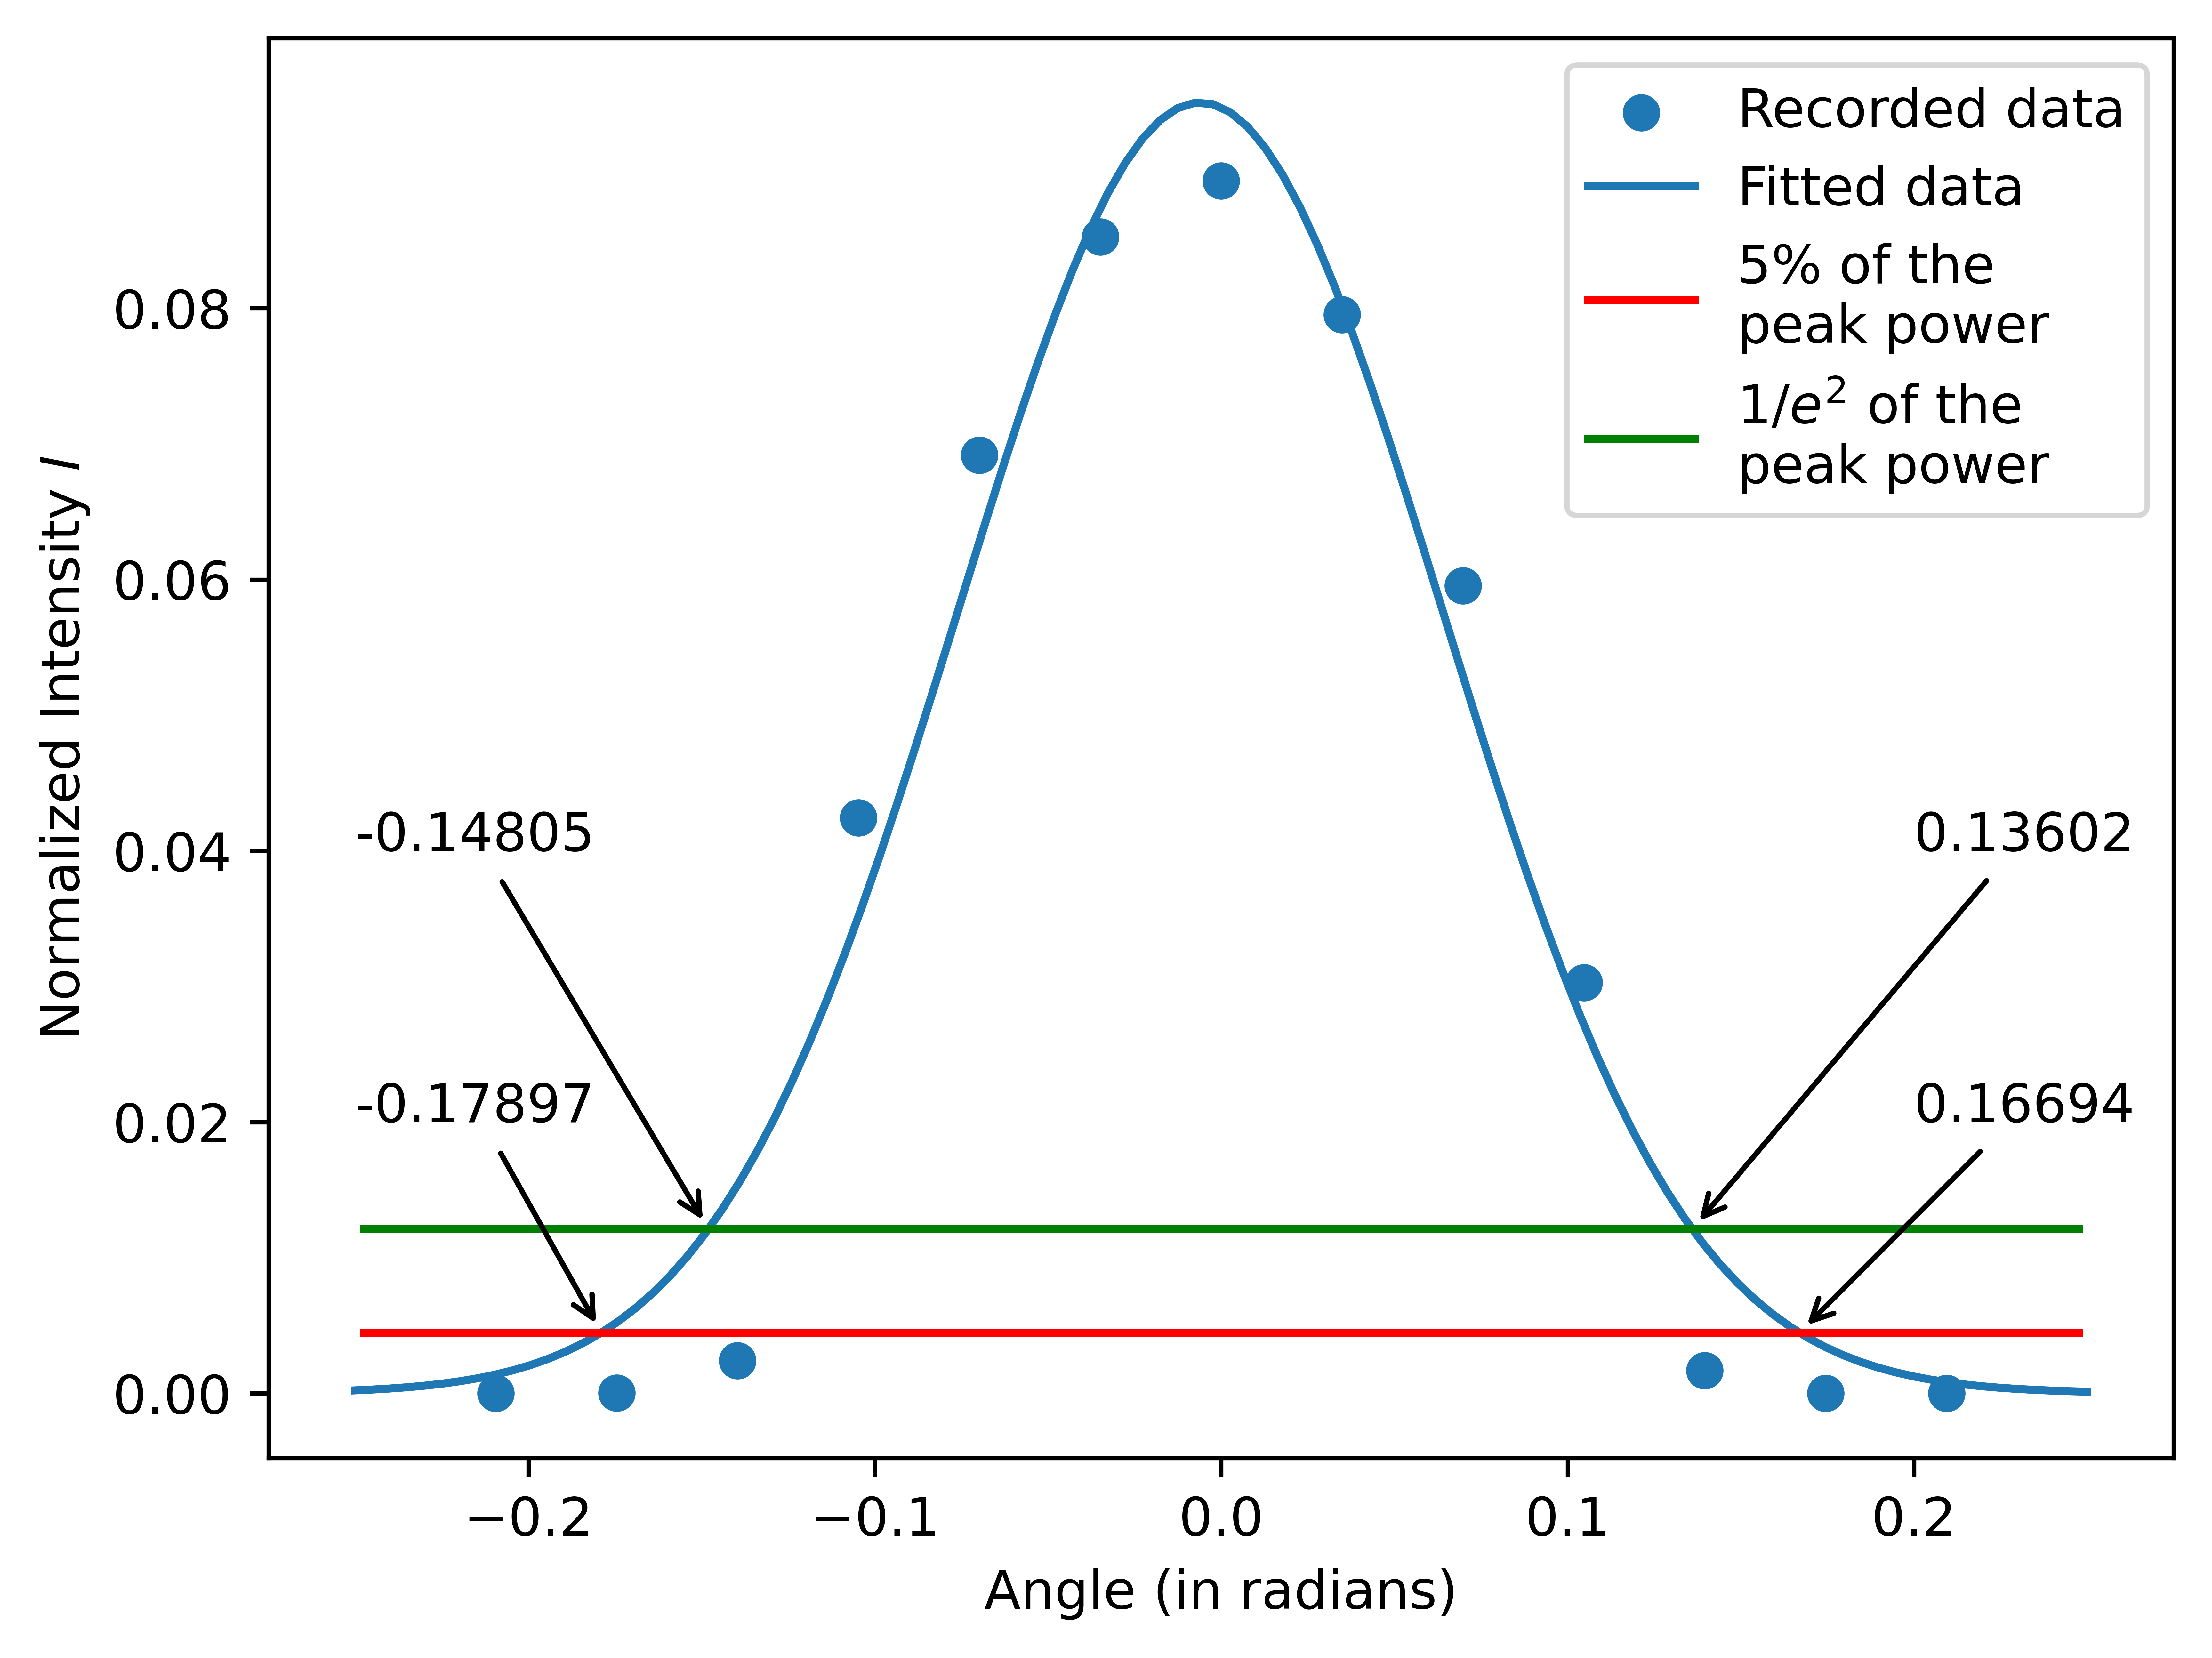
\includegraphics[scale = 0.56]{singlemodeNA}
	\caption{Plot for single-mode numerical aperture and mode-field diamter calculation}
	\label{fig:smNA}
\end{figure}
% Please add the following required packages to your document preamble:
% \usepackage{booktabs}
\begin{table}[]
	\caption{Recorded data for single-mode fiber numerical aperture measurement}
	\label{tab:smNA}
	\setlength{\tabcolsep}{10pt}
	\begin{tabular}{@{}cccc@{}}
		\toprule
		\begin{tabular}[c]{@{}c@{}}Angle\\ (in degrees)\end{tabular} & \begin{tabular}[c]{@{}c@{}}Angle \\ (in radians)\end{tabular} & \begin{tabular}[c]{@{}c@{}}Voltage $ V $\\ (in volts)\end{tabular} & \begin{tabular}[c]{@{}c@{}}Normalized \\ Intensity\\ ($ \propto V^2 $)\end{tabular} \\ \midrule
		-12                                               & -0.209                                             & 0                                               & 0.0000                                                     \\
		-10                                               & -0.175                                             & 0.004                                           & 0.0002                                                     \\
		-8                                                & -0.140                                             & 0.049                                           & 0.0269                                                     \\
		-6                                                & -0.105                                             & 0.206                                           & 0.4747                                                     \\
		-4                                                & -0.070                                             & 0.263                                           & 0.7737                                                     \\
		-2                                                & -0.035                                             & 0.292                                           & 0.9537                                                     \\
		0                                                 & 0.000                                              & 0.299                                           & 1.0000                                                     \\
		2                                                 & 0.035                                              & 0.282                                           & 0.8895                                                     \\
		4                                                 & 0.070                                              & 0.244                                           & 0.6659                                                     \\
		6                                                 & 0.105                                              & 0.174                                           & 0.3387                                                     \\
		8                                                 & 0.140                                              & 0.041                                           & 0.0188                                                     \\
		10                                                & 0.175                                              & 0.003                                           & 0.0001                                                     \\
		12                                                & 0.209                                              & 0                                               & 0.0000                                                     \\ \bottomrule
	\end{tabular}
\end{table}
% Please add the following required packages to your document preamble:
% \usepackage{booktabs}



\subsubsection{Multi-mode fiber}
For multi-mode fiber, we realized that the source we had will not work because to measure the numerical aperture for the multi-mode fiber, we need to excite all the guided modes approximately equally by means of an incoherent Lambertian source\footnote{A Lambertian source is an optical source which obeys the Lambertian cosine law which states hat the radiant intensity or luminous intensity observed from an ideal diffusely reflecting surface or ideal diffuse radiator is directly proportional to the cosine of the angle $ \theta $ between the direction of the incident light and the surface normal; $ I = I_0\cos(\theta) $.}, such as a tungsten halogen lamp (which unfortunately we could not obtain). It can be
shown that the power accepted at any point $ r $ in the fiber core from a Lambertian
source is directly proportional to square of the local numerical aperture.

Therefore, here we used the visual method to measure the numerical aperture and for the incoherent source, we employed a white light source. The reading are tabulated in Table \ref{tab:mmNA}. We recorded $ D = 2r $ versus $ z $ with the sources and used the following formulae
\begin{equation}\label{key}
	NA = \sin i_m = \sin[\tan^{-1}(D/2z)]
\end{equation}
After recording the values, we calculated the average value of NA as 0.2310 which is close to the actual value of 0.2.
% Please add the following required packages to your document preamble:
% \usepackage{booktabs}
% \usepackage{multirow}
\begin{table}[]
	\caption{Recorded data for multi-mode numerical aperture calculation}
	\label{tab:mmNA}
	\setlength{\tabcolsep}{12pt}
	\begin{tabular}{@{}ccccc@{}}
		\toprule
		$ z $ (in) & $ z $ (cm)  & $ r $ (cm) &  NA  &            Average NA             \\ \midrule
		2      & 5.08  & 1.3  & 0.2479 & \multirow{6}{*}{0.2310} \\
		3      & 7.62  & 1.8  & 0.2299 &                         \\
		5      & 12.7  & 3.1  & 0.2371 &                         \\
		6      & 15.24 & 3.6  & 0.2299 &                         \\
		7      & 17.78 & 4.1  & 0.2247 &                         \\
		8      & 20.32 & 4.5  & 0.2162 &                         \\ \bottomrule
	\end{tabular}
\end{table}
\subsection{Mode field diameter of a single-mode fiber}
\begin{figure}
	\centering
	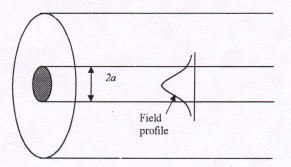
\includegraphics[scale = 0.7]{mfd}
	\caption{Schematic diagram of the amplitude distribution of the propagating fundamental
		mode ina single-mode fiber}
	\label{fig:mfd}
\end{figure}

The mode field diameter (MFD) is a measure of the optical power per unit area, across the end face of a single-mode
fiber. The most fundamental mode of the optical fibre is
$ LP_{01} $ mode which can be approximated to have a Gaussian
profile under the approximation of strong coupling. For any
Gaussian beam, the spread is calculated by FWHM (full width half maximum) angle.
The angle $ \theta_e $ at which the far-field intensity drops down by
a factor of $ e^2 $ from its maximum value at $ \theta = 0 $ would then
be given by:
\begin{equation}\label{key}
	\tan \theta_e = \dfrac{\lambda}{\pi w_0}
\end{equation}
which gives
\begin{equation}\label{key}
	w_0 (\textrm{mode field radius}) = \dfrac{\lambda}{\pi \tan \theta_e}
\end{equation}
\subsubsection*{\textbf{General Procedure}}
Same steps as measurement of NA of Multimode fibre,
with only one difference that at the ends of the single mode
fibre we put a few drops of oil to prevent cladding modes.
\subsubsection*{\textbf{Results}}
As annotated in the Figure \ref{fig:smNA}, the $ 1/e^2 $ value was found the angles $ \theta_1 = -0.14805 $ and $ \theta_2 = 0.13602 $. Therefore
\begin{equation}\label{key}
	\theta_e = \dfrac{0.14805+0.13602}{2} = 0.142035
\end{equation}
which gives $ \tan \theta_e = 0.143 $ and finally we get
\begin{equation}\label{key}
	w_0 = \dfrac{\lambda}{\pi \tan \theta_e} = \dfrac{\SI{632.8}{\nano \meter}}{\pi \times 0.143} = \SI{1.4}{\micro \meter}
\end{equation}
\subsection{Microbending loss in a multi-mode fiber}
In this experiment, we study intensity variation through a
fiber by inducing microbends in the fiber through a periodic
deformer element. When a portion of a fiber lay is sandwiched between two deformers and pressure is applied to
one of these deformer, the fiber undergoes periodic deformation in the form of micro-bends. The resultant mechan-
ical deformation of the optical fiber perpendicular to its
axis causes higher-order guided modes to radiate out of the
fiber’s core through the core-cladding interface as shown in
the figure. This results in a drop of intensity of the transmitted light through the fiber with increasing deformation.
\begin{figure}
	\centering
	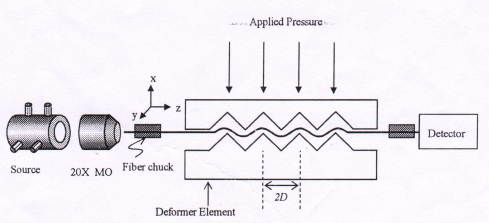
\includegraphics[scale = 0.6]{mbschematic}
	\caption{Experimental set-up for a simple intensity modulated fiber optic pressure
		sensor using a multi-mode fiber}
	\label{fig:mbschematic}
\end{figure}
\begin{figure}
	\centering
	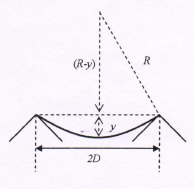
\includegraphics[scale = 0.7]{geometry}
	\caption{Geometry of the microbend}
	\label{fig:geometry}
\end{figure}
The loss is given as
\begin{equation}\label{key}
	\textrm{Loss} = C \Big(\dfrac{a}{R}\Big)^2
\end{equation}
From Figure \ref{fig:geometry}, 
\begin{equation}\label{key}
	R = \dfrac{y^2 + D^2}{2y}
\end{equation}
where $ y $ is the displacement of the deformer element and $ 2D $ is the distance between the
contact points of the deformer element, which is equal to the pitch of the element. Thus,
the transmittance $ T $ through the fiber is
\begin{equation}\label{key}
	T = 1 - \textrm{Loss} = 1 - \dfrac{Ca^2}{\Bigg(\dfrac{y^2 + D^2}{2y}\Bigg)^2}
\end{equation}
or
\begin{equation}\label{eq:microbending}
	T = 1 - C' \Bigg(\dfrac{q}{1+q^2}\Bigg)^2
\end{equation}
where $ C' = 4Ca^2/D^2 $ and $ q = y/D $. The applied force and hence the pressure is proportional to the displacementy. Therefore
in terms of pressure, we have
\begin{equation}\label{key}
	q = \dfrac{PA}{kD} = \dfrac{mg}{kD}
\end{equation}
where $ P $ is the pressure, $ A $ is the surface area of the deformer $ mg $ is the weight and $ k $ is a constant. 
\subsubsection*{\textbf{General Procedure}}
\begin{enumerate}
	\item We sandwich the fibre between two periods which will
	help induce microbending.
	\item A weight pan is placed on top of the period
	\item Weight on the pan is gradually increased and the cor-
	responding value for the intensity is noted.
\end{enumerate}
\subsubsection*{\textbf{Results}}
The results and the data recorded is tabulated in Table \ref{tab:microbend} and is plotted and fitted in Figure \ref{fig:microbending}. After fitting the recorded data with equation \ref{eq:microbending}, we obtained $ C' = 8.489 $ and $ q = Ax = 5.588 \times 10^{-4} $ where $ A = g/kD $.
% Please add the following required packages to your document preamble:
% \usepackage{booktabs}
\begin{table}[]
	\caption{Recorded data for microbending loss in multi-mode fiber}
	\label{tab:microbend}
	\setlength{\tabcolsep}{24pt}
	\begin{tabular}{@{}ccc@{}}
		\toprule
		\begin{tabular}[c]{@{}c@{}}Mass\\ (in grams)\end{tabular} & \begin{tabular}[c]{@{}c@{}}Voltage\\ (in volts)\end{tabular} & \begin{tabular}[c]{@{}c@{}}Normalized \\ Intensity\end{tabular} \\ \midrule
		0      & 0.325 & 1      \\
		106.17 & 0.291 & 0.8017 \\
		203.37 & 0.279 & 0.7370 \\
		299.73 & 0.276 & 0.7212 \\
		387.91 & 0.253 & 0.6060 \\
		486.68 & 0.247 & 0.5776 \\
		580.2  & 0.18  & 0.3067 \\
		675.58 & 0.046 & 0.0200 \\ \bottomrule
	\end{tabular}
\end{table}
\begin{figure}
	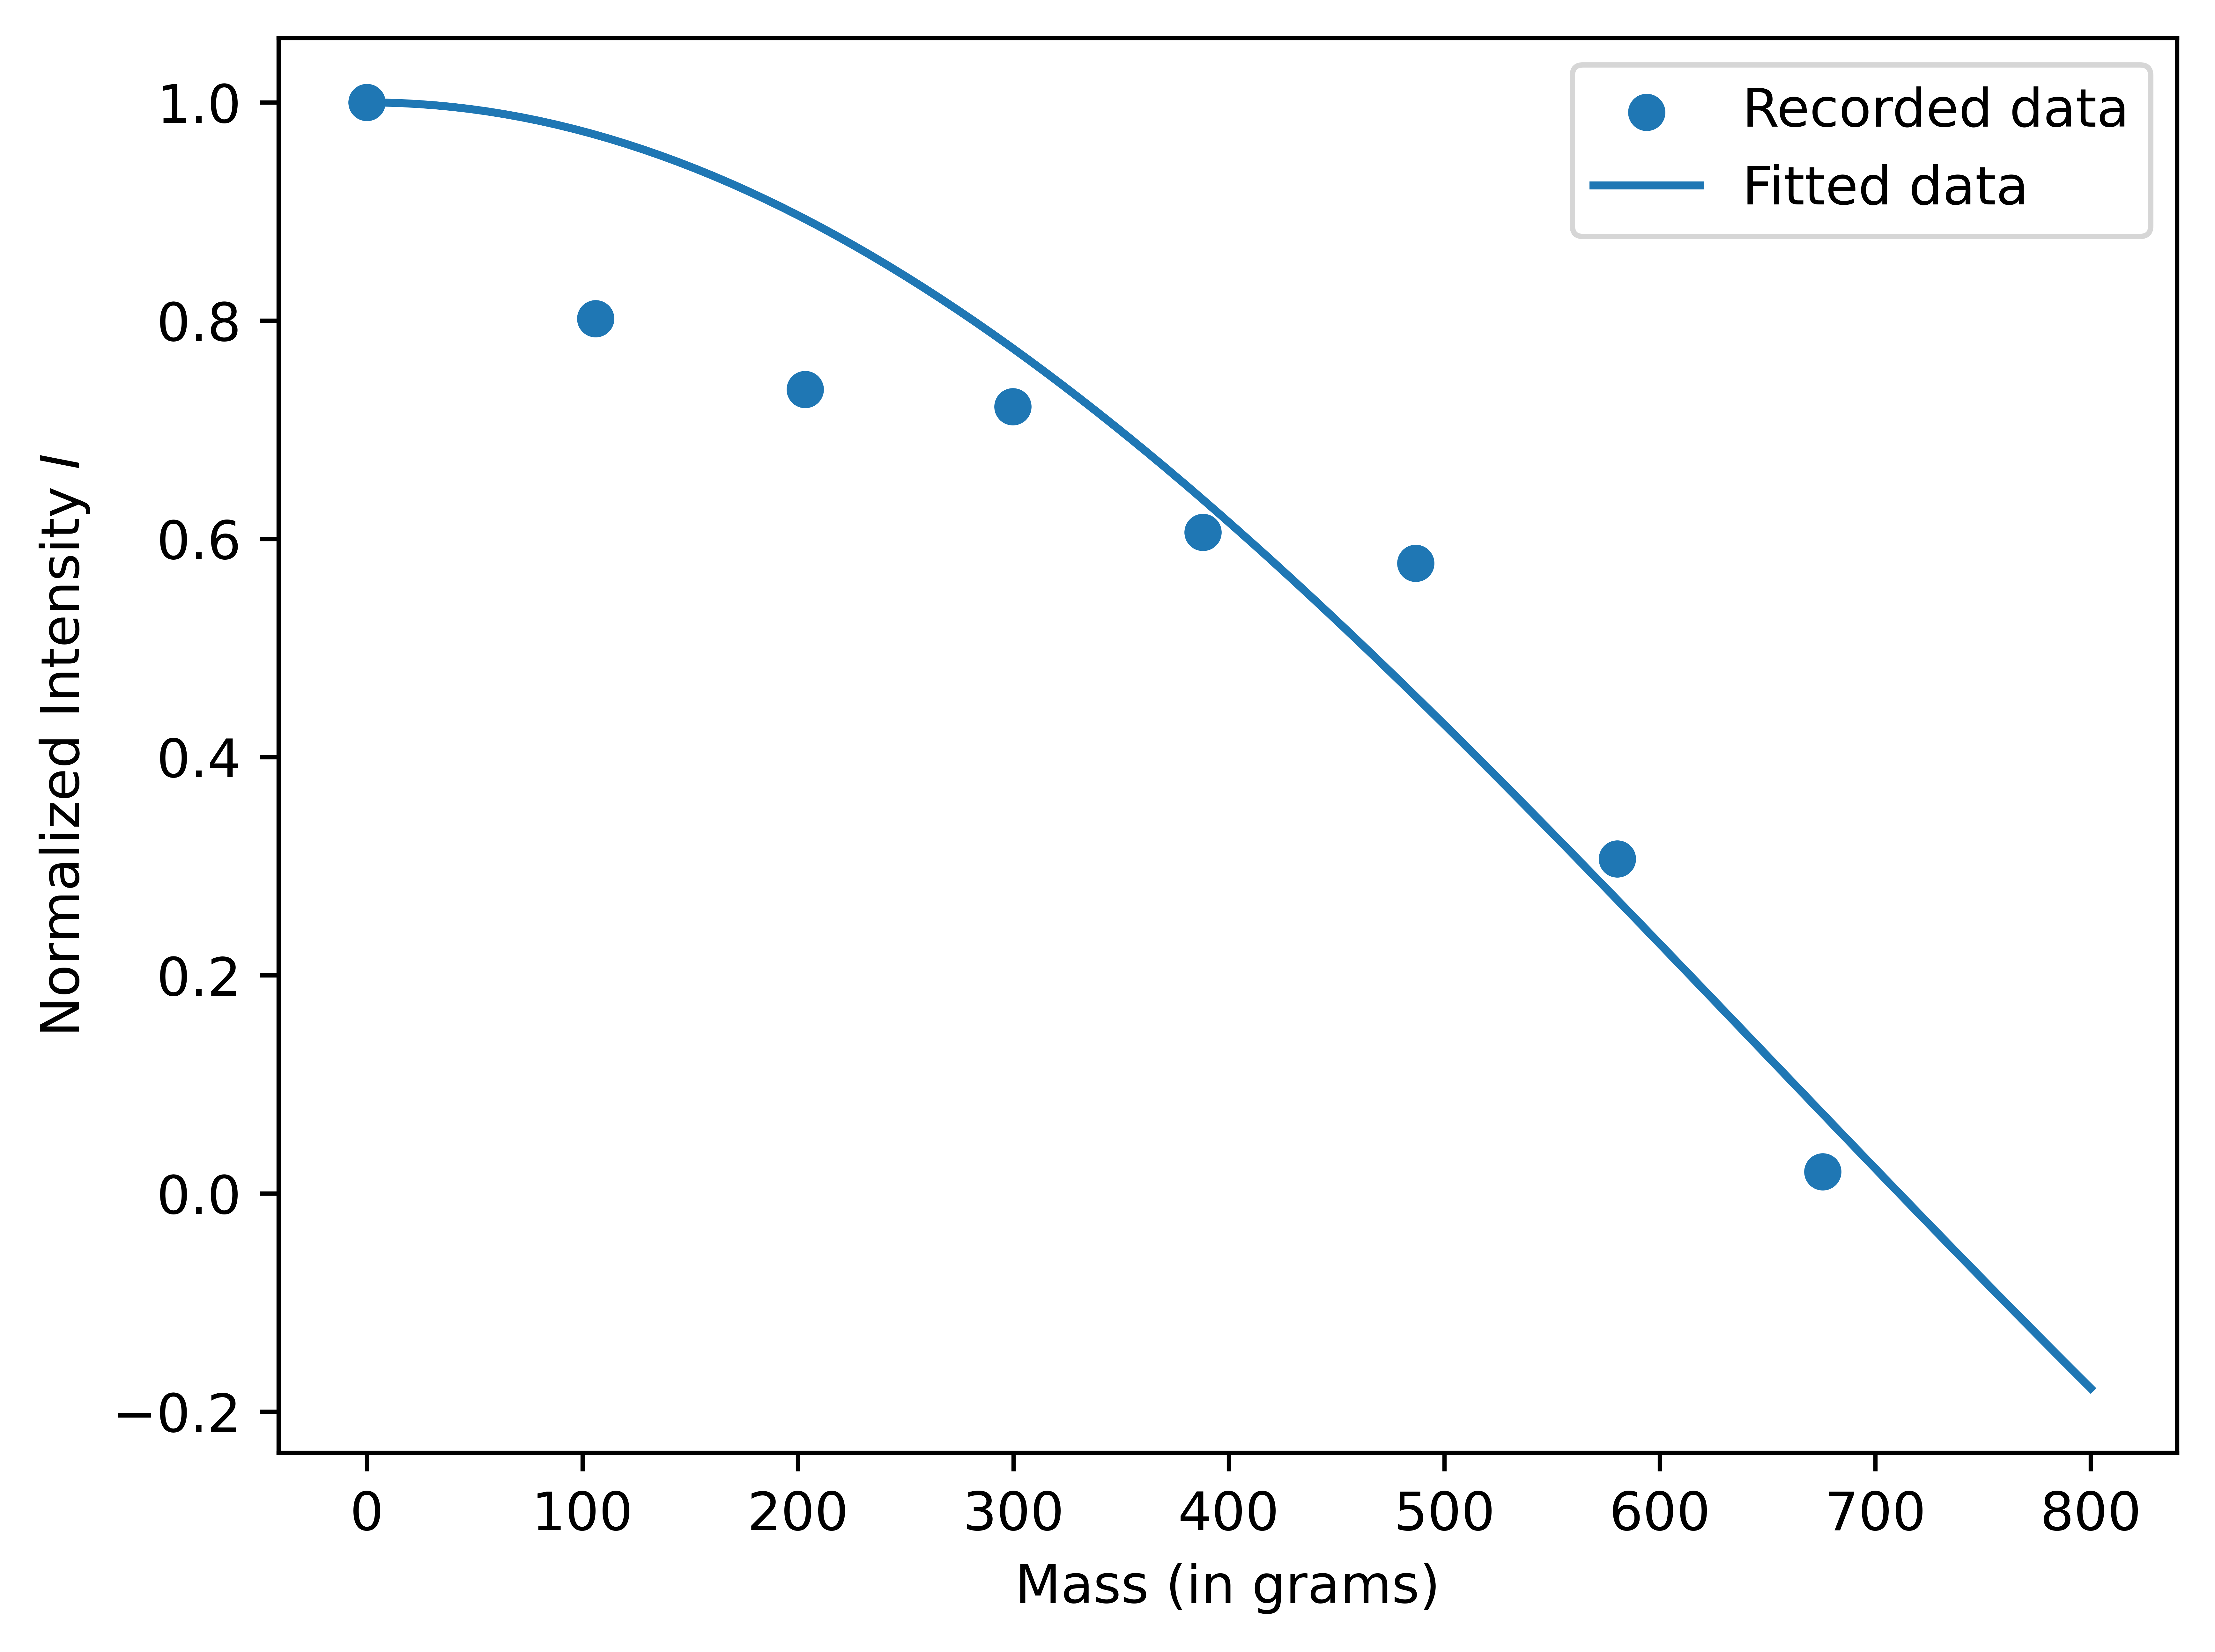
\includegraphics[scale =0.56]{microbending}
	\caption{Amount of light transmitted through a microbend-modulated fiber-optic sensor
		versus the applied weight.}
	\label{fig:microbending}
\end{figure}
\subsection{Bend-induced loss in a single-mode fiber}
The bending loss can be accounted for by the transition
losses and the macrobend losses. Transition loss is due to
the abrupt changes in curvature occurring, at the cross sectional plane of the fiber. The predominant effect of curvature on the fundamental mode is to shift the peak of the field
distribution radially outwards (in the plane of the bend) by
a distance $ r_d $ from the fiber axis.

The second mechanism of loss is the actual transmission
loss suffered due to radiation from side of the bent fiber.The
evanescent tail in the cladding decays almost exponentially
with distance from the core-cladding interface. Since the
evanescent tail moves along with the field in the core, part
of the energy of a propagating mode travels in the fiber
cladding.

The pure bend loss coefficient (in dB per unit length of
the bent fiber) in a single moded step index fiber is given by:
\begin{equation}\label{key}
	\alpha \approx 4.34 \Bigg(\dfrac{\pi}{4aR_c}\Bigg)^{1/2} \Bigg(\dfrac{U}{V K_1(W)}\Bigg)^2 \dfrac{1}{W^{3/2}} \exp \Big(-\dfrac{4}{3} \dfrac{R_c}{a} \dfrac{W^3 \Delta}{V^2}\Big)
\end{equation}
Here $ K_1(x) $ is is the modified Bessel function of second kind. The
parameters $ U $ , $ W $, $ V $ and $ \Delta $ are defined through:
\begin{center}
	$ U = a \sqrt{k_0^2 n_1^2 - \beta^2} $ \\
	$ W = a \sqrt{\beta^2 - k_0^2 n_2^2}$ \\
	$ V^2 = U^2 + W^2 $ \\
	$ \Delta \simeq (n_1 - n_2)/n_2 $ \\
	$ k_0 = 2 pi/ \lambda $
\end{center}
We wind the fibre around the spool and the absorption coefficient ($ \alpha $) is given by:
\begin{equation}\label{key}
	\alpha = -\dfrac{10}{L} \log \dfrac{P_2}{P_1}
\end{equation}
where $ L $ is the length of the fiber (within the bend) i.e.
$ 2\pi R \times $ (no. of turns), $ P_1 $ is the output power without the
bend in the fiber and $ P_2 $ is the output power with the bend
in the fiber.

We compare our curve to given theoretical equation:
\begin{equation}\label{key}
	\alpha = 1187.3 \exp(-10.3941*R)/R^{0.5}
\end{equation}
\subsubsection*{\textbf{General Procedure}}
\begin{enumerate}
	\item After coupling the fibre to the 20X microscope, we
	measure the maximum output through the detector
	\item Then the optical fibre is wound on the top of the
	first spool. First a single turn is done and output is
	recorded. Other objects such as brass rod, or pen were
	also used to induce bends.
	\item Then the process is repeated on the larger radius sec-
	tion of the spool.
	\item The data is fitted to the given theoretical curve.
\end{enumerate}
\subsubsection*{\textbf{Results}}
We recorded and tabulated the data in Table \ref{tab:bendloss} and plotted and fitted the data in Figure \ref{fig:bendloss1}.
\begin{figure}
	\centering
	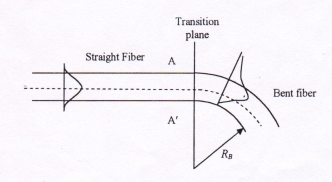
\includegraphics[scale = 0.65]{bend1}
	\caption{A qualitative representation of the shift in the Gaussian-like fundamental mode
		away from the fiber axis at a bend.}
	\label{fig:bend1}
\end{figure}
\begin{figure}
	\centering
	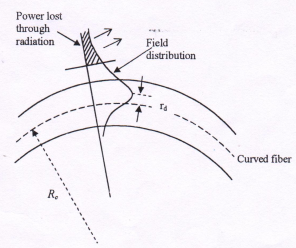
\includegraphics[scale=0.65]{bend2}
	\caption{Schematic representation of the bending loss in a section of fiber bent into an arc of radius $ R_c $}
	\label{fig:bend2}
\end{figure}
\begin{figure}
	\centering
	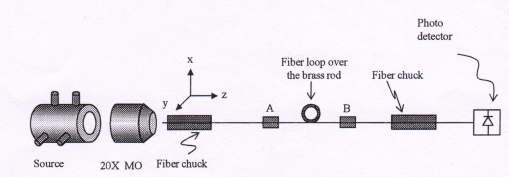
\includegraphics[scale=0.65]{bend3}
	\caption{Experimental setup to study the macro-bending loss in a single mode fiber}
	\label{fig:bend3}
\end{figure}
\begin{figure}
	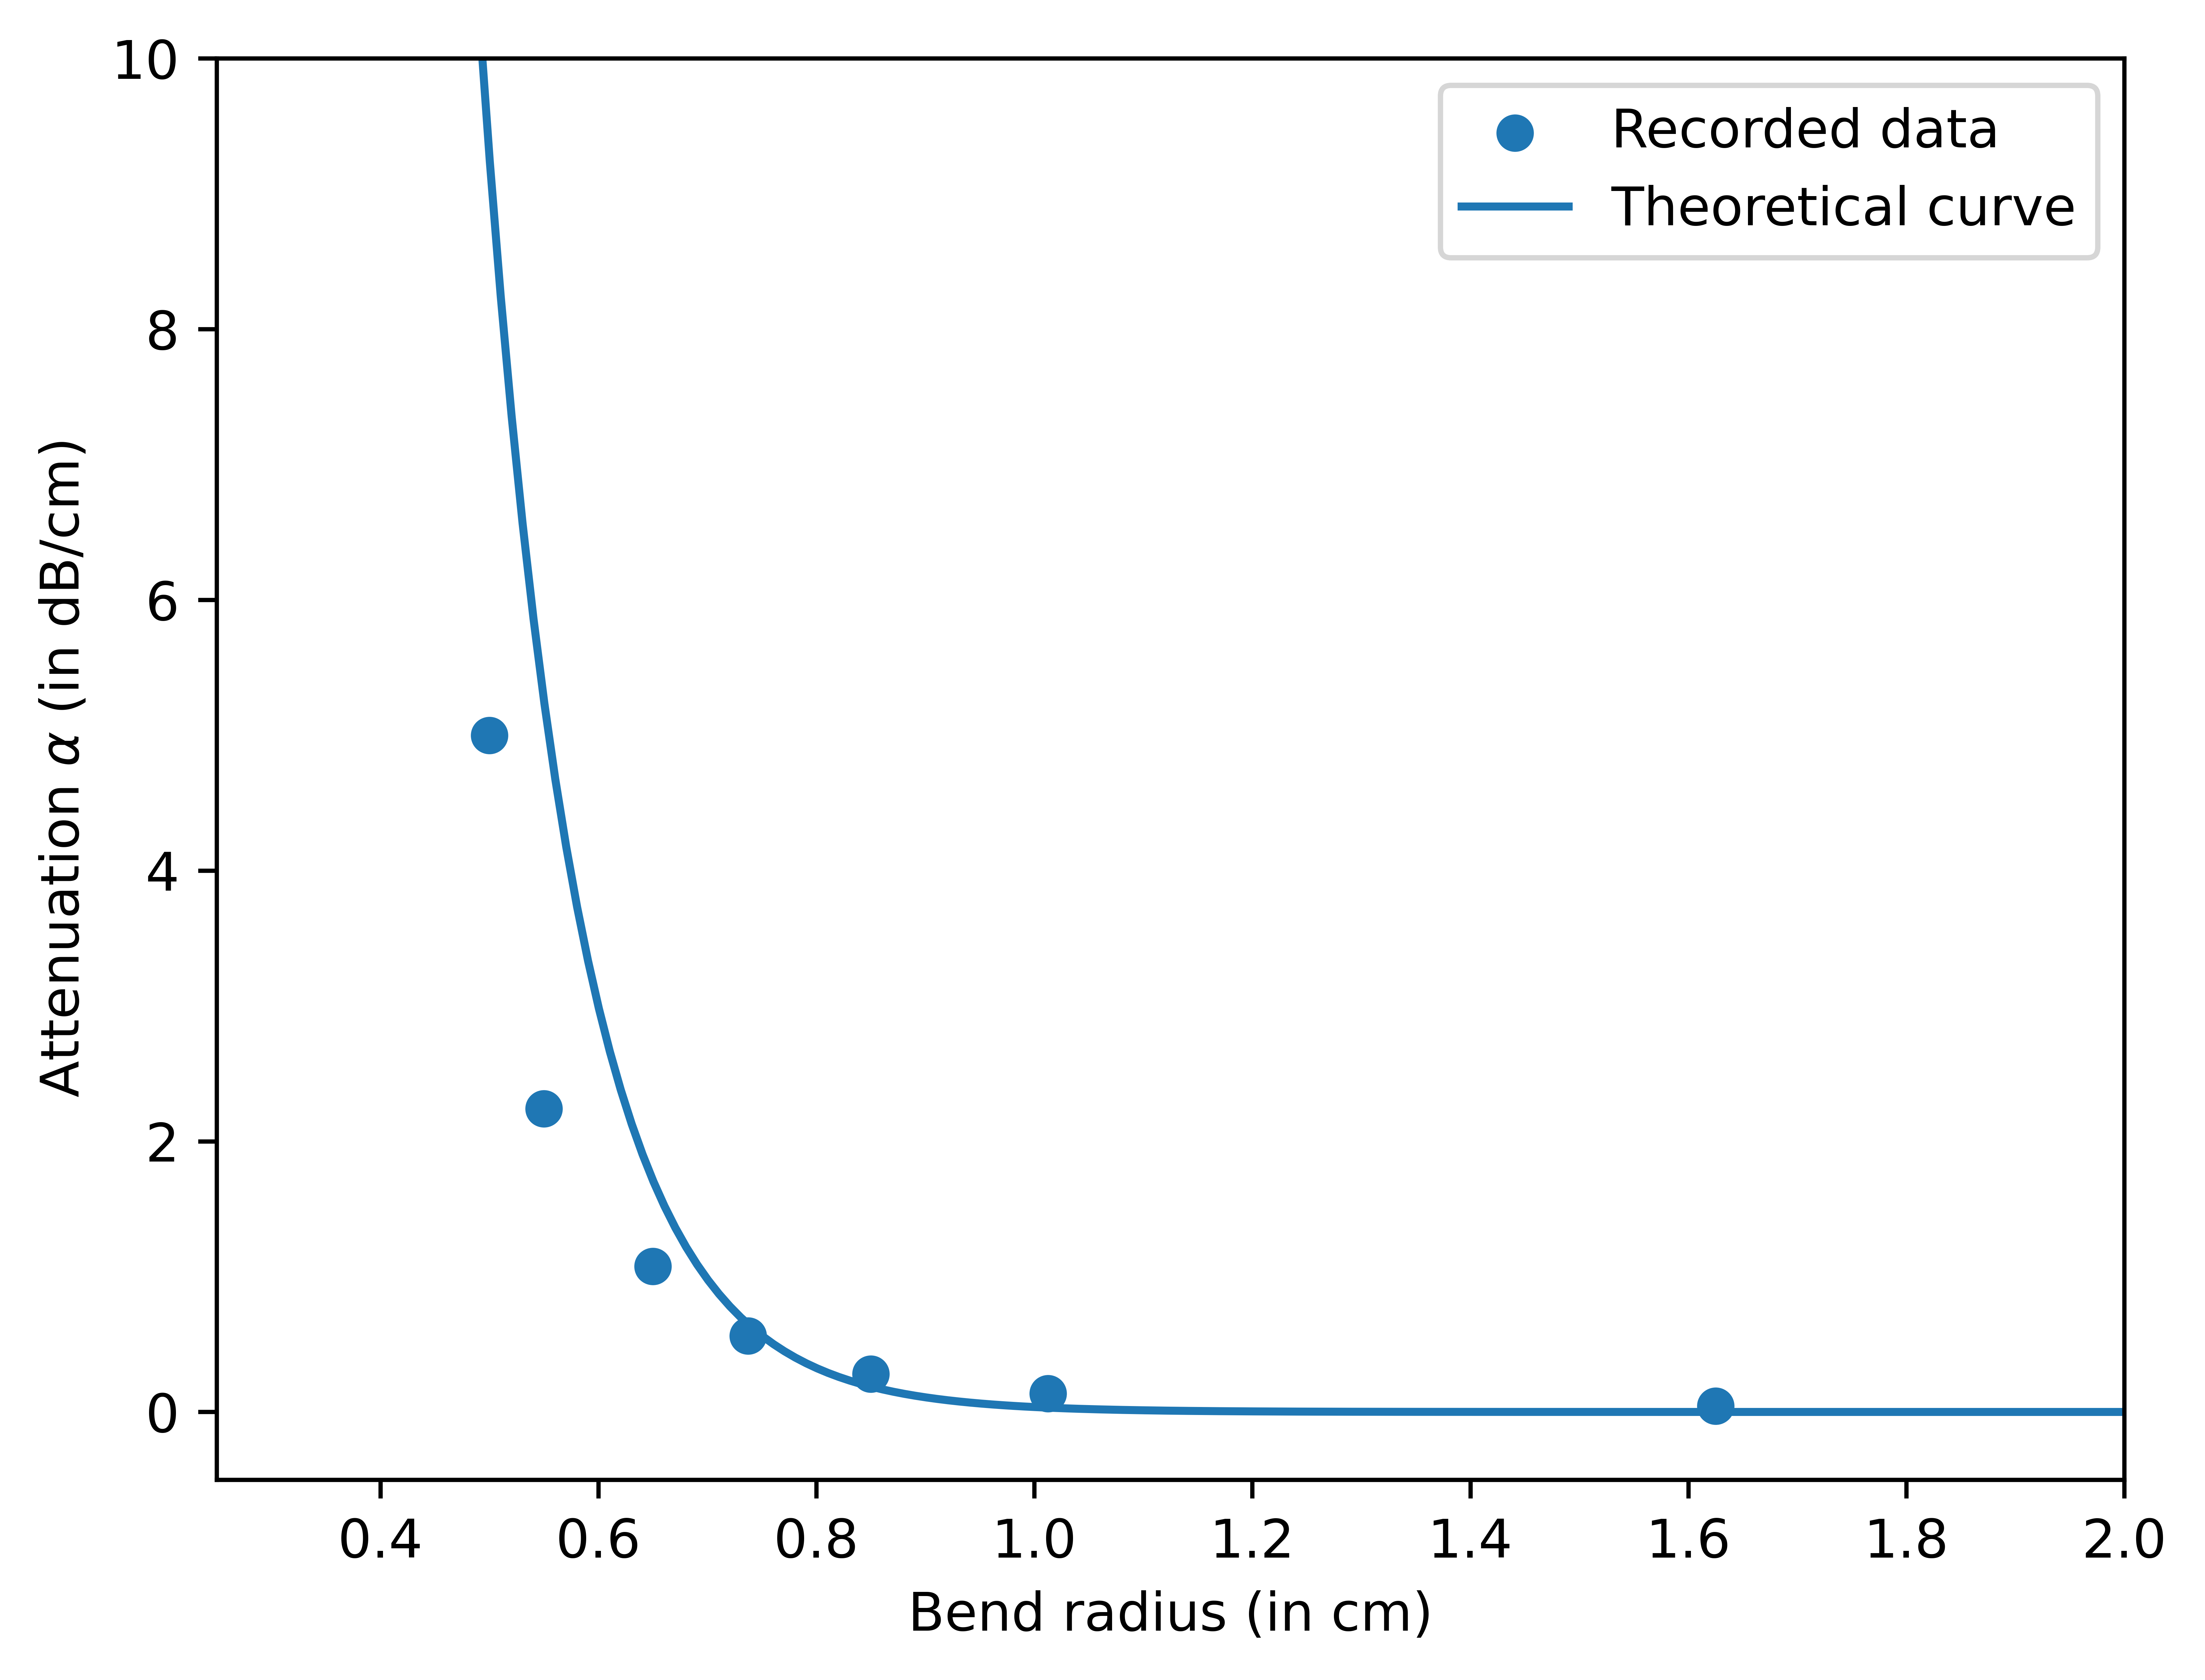
\includegraphics[scale=0.56]{bendloss}
	\caption{Bend loss of a single mode step-index fiber as a function of bend radius.}
	\label{fig:bendloss1}
\end{figure}
% Please add the following required packages to your document preamble:
% \usepackage{booktabs}
\begin{table*}[]
	\caption{Recorded data for bend-induced loss in single-mode fiber}
	\label{tab:bendloss}
	\setlength{\tabcolsep}{8pt}
	\begin{tabular}{@{}ccccccc@{}}
		\toprule
		\begin{tabular}[c]{@{}c@{}}Diameter $ D $\\ (in cm)\end{tabular} &
		\begin{tabular}[c]{@{}c@{}}Radius $ r = D/2$\\ (in cm)\end{tabular} &
		\begin{tabular}[c]{@{}c@{}}Bend length ($ L = 2 \pi r $)\\ (in cm)\end{tabular} &
		\begin{tabular}[c]{@{}c@{}}Voltage $ V $\\ (in volts)\end{tabular} &
		\begin{tabular}[c]{@{}c@{}}Voltage loss $ \Delta V $\\ $ V/V_{max}\ $ \end{tabular} &
		\begin{tabular}[c]{@{}c@{}}Power loss $ \Delta P $\\ ($ \propto (\Delta V)^2 $)\end{tabular} &
		\begin{tabular}[c]{@{}c@{}}Attenuation $ \alpha $\\ (in dB/cm)\end{tabular} \\ \midrule
		1.000 & 0.5000 & 3.142  & 0.062 & 0.164 & 0.027 & 4.998 \\
		1.100 & 0.5500 & 3.456  & 0.155 & 0.410 & 0.168 & 2.241 \\
		1.300 & 0.6500 & 4.084  & 0.228 & 0.603 & 0.364 & 1.075 \\
		1.475 & 0.7375 & 4.634  & 0.280 & 0.741 & 0.549 & 0.563 \\
		1.700 & 0.8500 & 5.341  & 0.318 & 0.841 & 0.708 & 0.281 \\
		2.025 & 1.0125 & 6.362  & 0.342 & 0.905 & 0.819 & 0.137 \\
		3.250 & 1.6250 & 10.210 & 0.359 & 0.950 & 0.902 & 0.044 \\ \bottomrule
	\end{tabular}
\end{table*}
\section{Results, Discussions and Conclusions} \label{sec:Disc}
\begin{enumerate}
	\item The numerical aperture for single-mode fiber was calculated to be 0.172.
	\item The numerical aperture for multi-mode fiber was calculated to be 0.2310. 
	\item The mode-field diameter of the single-mode fiber was calculated to be $ \SI{1.4}{\micro \meter} $.
	\item We successfully studied and fitted the trend for microbending loss in a multi-mode fiber.
	\item We successfully studied and fitted the trend for bend-induced loss in a single-mode fiber.
	\item In a multimode fiber, different mode groups suffer different attenuation rates, which is
	referred to as differential mode attenuation (DMA). Therefore the NA measured by visual means is generally a bit inflated.
	\item In addition, NA is
	critically dependent on the excitation conditions. To ensure that all the guided modes are
	excited in a multimode fiber, an "overfill launch" is applied at the input end i.e. one uses
	a microscope objective of NA higher than that of the fiber for launching light into the
	fiber. This results in the excitation of the cladding modes and the radiation modes, which
	quickly lose power as they propagate along the fiber.
	\item he analyses discussed under the theory section are based on meridional rays.
	However, a greater power loss arises when skew rays are included in the analyses, since
	many of the skew rays that geometric optics predicts are trapped in the fiber are actually
	leaky rays. These leaky rays are only partially confined to the core of the circular optical
	fiber and attenuate as the light travels along the fiber. Thus, a detailed inclusion of skew
	rays will change the expression of the light acceptance ability (NA) of the fiber.
	\item It is necessary that the far-field intensity pattern be detected at a sufficiently large
	distance from the center of the fiber output end such that good angular resolution is
	achieved in detection.
	\item Fiber optics also provided a revolutionary
	technology base for configuring a variety of optical sensors, which offer several!
	advantages over existing traditional sensing techniques. These optical sensors are direct consequences of the physical effects we studied through micr-bending loss.
	\item  One of the most
	important parameters in determining the microbending sensitivity is the periodicity of the
	fiber deformation. To understand this, one has to consider the mode coupling effects in
	fibers.
\end{enumerate}
	

\section{Precautions}
\begin{enumerate}
	\item The fiber end faces must be of good quality.
	\item Cladding-mode strippers must be used.
	\item The output end of the fiber must be positioned in such a way that the axis
	of the rotation of rotation stage passes through it.
	\item The two plates of the deformer must be accurately aligned.
\end{enumerate}

	

	
	


\appendix

% The \nocite command causes all entries in a bibliography to be printed out
% whether or not they are actually referenced in the text. This is appropriate
% for the sample file to show the different styles of references, but authors
% most likely will not want to use it.
%\nocite{*}

%bibliography{apssamp}% Produces the bibliography via BibTeX.

\end{document}
%
% ****** End of file apssamp.tex ******
